\documentclass[letterpaper,9pt,twocolumn,twoside,]{pinp}

%% Some pieces required from the pandoc template
\providecommand{\tightlist}{%
  \setlength{\itemsep}{0pt}\setlength{\parskip}{0pt}}

% Use the lineno option to display guide line numbers if required.
% Note that the use of elements such as single-column equations
% may affect the guide line number alignment.

\usepackage[T1]{fontenc}
\usepackage[utf8]{inputenc}

% pinp change: the geometry package layout settings need to be set here, not in pinp.cls
\geometry{layoutsize={0.95588\paperwidth,0.98864\paperheight},%
  layouthoffset=0.02206\paperwidth, layoutvoffset=0.00568\paperheight}

\definecolor{pinpblue}{HTML}{185FAF}  % imagecolorpicker on blue for new R logo
\definecolor{pnasbluetext}{RGB}{101,0,0} %


\usepackage{leading}
\leading{0pt}

\title{House Prices in New York City}

\author[]{Ishaan Syed Zahiruddin \textbar{} Jonah Smith \textbar{} Kunal
Ostwal \textbar{} Luke Gallagher \textbar{} Yibo Zhao}


\setcounter{secnumdepth}{0}

% Please give the surname of the lead author for the running footer
\leadauthor{}

% Keywords are not mandatory, but authors are strongly encouraged to provide them. If provided, please include two to five keywords, separated by the pipe symbol, e.g:
 \keywords{  Regression models |  Stepwise AIC |  NYC Real Estate  }  

\begin{abstract}
The goal was to find the possible price prediction for each of the
houses. To find features of the dataset that may have a strong
correlation with Price, a heat map of the correlation between each pair
of variables was generated. The heatmap showed us that Bathrooms, Rooms
and Land.Value have a Strong correlation coefficient with Price.
Living.Area had the greatest correlation coefficient with Price while
Age has a small relationship with Price. With the help of a simple
linear model between Living.Area and Price and a multi-variate model
where we used both the Forward Stepwise Function(FSF) and Backward
Stepwise Function(BSF) which produced the same model. In sample
performance showed us that multivariate model has a better goodness of
fit compared to the univariate model. 10-fold cross validation test
confirmed our findings. From the top three variables with the strongest
ability to predict housing price, Price and Living.Area had the highest
correlation relationship. This meant that the size of the property
increased the price.
\end{abstract}

\dates{This version was compiled on \today} 


% initially we use doi so keep for backwards compatibility
% new name is doi_footer
\doifooter{CC08E2}

\pinpfootercontents{New York Housing Data}

\begin{document}

% Optional adjustment to line up main text (after abstract) of first page with line numbers, when using both lineno and twocolumn options.
% You should only change this length when you've finalised the article contents.
\verticaladjustment{-2pt}

\maketitle
\thispagestyle{firststyle}
\ifthenelse{\boolean{shortarticle}}{\ifthenelse{\boolean{singlecolumn}}{\abscontentformatted}{\abscontent}}{}

% If your first paragraph (i.e. with the \dropcap) contains a list environment (quote, quotation, theorem, definition, enumerate, itemize...), the line after the list may have some extra indentation. If this is the case, add \parshape=0 to the end of the list environment.


\hypertarget{introduction}{%
\subsection{Introduction}\label{introduction}}

The USA was hit hard by the COVID pandemic and New York City in
particular was the hardest hit city worldwide. The goal of our project
was to find the best possible price prediction for each of the houses.
The dependent variable was Price of the house. A preliminiary look at
the dataset showed us that the New York real estate market is a buyer's
market with total sales to listing ratio of 0.12 i.e.~the supply of
homes is much higher than the demand for homes. Hence, it is a buyer's
market.

\hypertarget{dataset-description}{%
\subsection{Dataset Description}\label{dataset-description}}

The dataset used by us is a random sample of houses from a much larger
dataset called the Saratoga Housing Data. The dataset has both
categorical and numerical variables which will help to make a more
comprehensive prediction. We take it for granted that the data has been
independently collected. Since it is a random sample of a larger
dataset, the data is assumed to be void of any comfounding factors
related to sampling and therefore, we assume there is independence
between error terms. Data Cleaning was not an ardous process as the
dataset used by us was cleaned by the authors. There were no empty
cells. There was an extra variable Test which is not a part of the
original Saratoga dataset. Since we do not have a description of it, we
omit it from our analysis to remove any comfounding factors from the
result.

\hypertarget{analysis}{%
\subsection{Analysis}\label{analysis}}

\hypertarget{simple-linear-model}{%
\subsubsection{Simple Linear Model}\label{simple-linear-model}}

There are a number features of the data set such as
\texttt{Living.Area}, \texttt{Age}, \texttt{Land.Value}, that seem like
they ought to prima facie have a strong correlation with \texttt{Price}.
Indeed, a heat map of the correlation between each pair of variables
shows a number of interesting things.

\begin{center}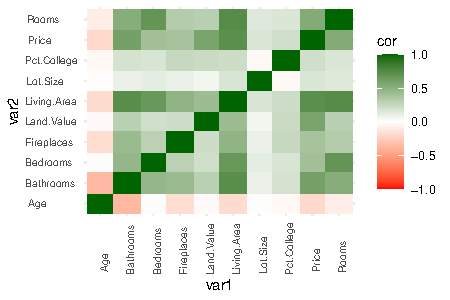
\includegraphics{DATA2002---Group-Project-Executive-Summary_files/figure-latex/unnamed-chunk-3-1} \end{center}

The features \texttt{Bathrroms}, \texttt{Rooms}, and \texttt{Land.Value}
all have a strong correlation coefficient with \texttt{Price}; -
surprisingly, \texttt{Age} has a small relationship with \texttt{Price};
- less suprisingly, \texttt{Living.Area} has the greatest correlation
coefficient with \texttt{Price} of \(0.71\).

\hypertarget{price-vs-living-area}{%
\paragraph{Price vs Living Area}\label{price-vs-living-area}}

\begin{center}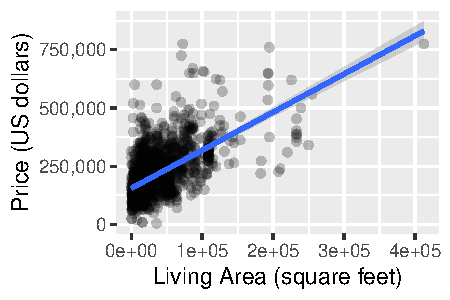
\includegraphics{DATA2002---Group-Project-Executive-Summary_files/figure-latex/unnamed-chunk-4-1} \end{center}

\begin{itemize}
\tightlist
\item
  Consequently, we decided to produce a simple linear model between
  \texttt{Living.Area} and \texttt{Price}, described by the equation
  \[\text{Price} = 12844.18 + 113.3729 * \text{Living.Area}\].\\
  \vspace{-8mm}
\end{itemize}

\hypertarget{stepwise-models}{%
\subsubsection{Stepwise Models}\label{stepwise-models}}

After looking at the result of the simple linear model, we generated a
stepwise model to test the dataset's performance in a complex model. We
tested both models: the forward and backward AIC function and ended up
with the same model. \begin{equation}
  \begin{aligned}
Price&=7740.54\ +\ 70.17\ * \text{Living.Area}\ +\ 0.92\ * \text{Land.Value} \\
&+\ \ensuremath{2.304818\times 10^{4}} * \text{Bathrooms} + \ensuremath{1.203278\times 10^{5}} * \text{Waterfront}\   \\
& \ensuremath{-4.454452\times 10^{4}} * \text{New.Construct} + 9998.56 * \text{Heat.Type(Hot Air)}\ \\
& -511.48 * \text{Heat.Type(Hot Water)}\ \ensuremath{-3.295233\times 10^{4}} * \text{Heat.Type(None)}\\
&+\ 7372.04 * \text{Lot.Size} - 9639.2 * \text{Central.Air}\\
& -140.8 * \text{Age} + 3045.91 * \text{Rooms}  -7797.56 * \text{Bedrooms}\\
       \label{eqn:example}
  \end{aligned}
\end{equation}

From the generated equation it can be seen that the following factors
were not added to the model by the FSF and were excluded by the BSF:
\texttt{Pct.College}, \texttt{Fireplaces}, \texttt{Fireplaces},
\texttt{Sewer.Type}, and \texttt{Fuel.Type}.

\hypertarget{performance-analysis}{%
\subsection{Performance Analysis}\label{performance-analysis}}

\hypertarget{in-sample-performance}{%
\subsubsection{In-sample Performance}\label{in-sample-performance}}

Here we compare the performance of the multivariate regression model to
that of the simple linear regression model within the dataset.
\begin{equation}
  \begin{aligned}
&\text{Simple Model}\ r^2: 0.5090615\\
&\text{Multivariate Model}\ r^2: 0.6548216
       \label{eqn:example}
  \end{aligned}
\end{equation}\\
Hence, the multivariate model has a better goodness of fit compared to
the univariate model.

\hypertarget{out-of-sample-performance}{%
\subsubsection{Out of Sample
Performance}\label{out-of-sample-performance}}

We chose Mean Absolute Error over Root Mean Square Error since there are
several outliers in the data.

We compared the mean absolute error of the two models.\\
\begin{equation}
  \begin{aligned}
&\text{MAE(Univariate Model):}\ 46975.15\\  
&\text{MAE(Multivariate Model):}\ 41735.76  
       \label{eqn:example}
  \end{aligned}
\end{equation}\\
The multivariate model has the lower mean absolute error, as such it is
better at predicting the prices of New York houses than the linear
model.

\hypertarget{fold-cross-validation}{%
\subsubsection{10-fold Cross Validation}\label{fold-cross-validation}}

We performed a 10-fold cross validation test on the two models.

\begin{center}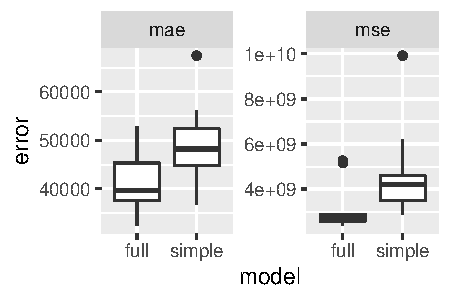
\includegraphics{DATA2002---Group-Project-Executive-Summary_files/figure-latex/unnamed-chunk-12-1} \end{center}

\hypertarget{assumptions}{%
\subsection{Assumptions}\label{assumptions}}

\hypertarget{for-univariate-model}{%
\paragraph{For Univariate model}\label{for-univariate-model}}

Linearity: The residuals plotted in the univariate model appear
symmetrically distributed above and below zero with some outliers above
zero, therefore the data is assumed to be linear.

\begin{center}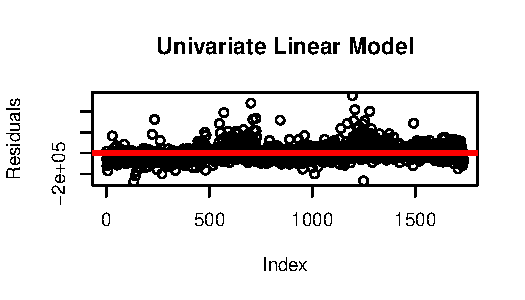
\includegraphics{DATA2002---Group-Project-Executive-Summary_files/figure-latex/unnamed-chunk-13-1} \end{center}

Homoskedacity: In the model,it appears the variance is constant in the
residuals plot for each error term and therefore the homoskedacity
assumption is satisfied.

\hypertarget{for-multivariate-model}{%
\paragraph{For Multivariate model:}\label{for-multivariate-model}}

\hypertarget{linearity}{%
\subsubsection{Linearity}\label{linearity}}

The residuals plotted in the multivariate model appear symmetrically
distributed above and below zero with some outliers above zero,
therefore the data is assumed to be linear.

\begin{center}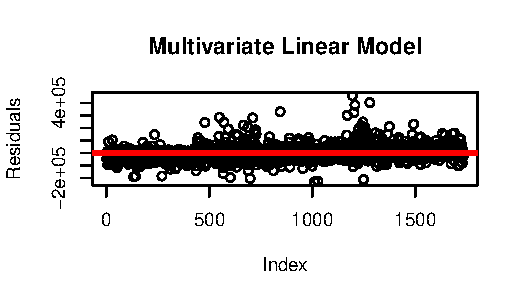
\includegraphics{DATA2002---Group-Project-Executive-Summary_files/figure-latex/unnamed-chunk-14-1} \end{center}

\hypertarget{homoskedacity}{%
\subsubsection{Homoskedacity}\label{homoskedacity}}

In the univariate model, it appears the variance is constant in the
residuals plot for each error term and therefore the homoskedacity
assumption is satisfied.

\hypertarget{normality}{%
\subsubsection{Normality}\label{normality}}

The majority of points lie close to the diagonal line in both QQ plots,
however, there are many outliers in the upper tail so the normality
assumption is moderately well satisfied.

\begin{center}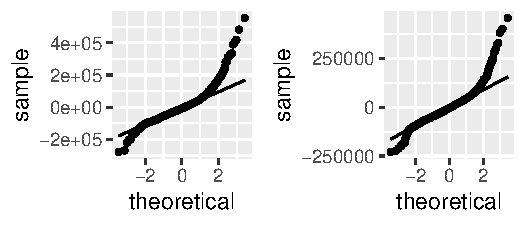
\includegraphics{DATA2002---Group-Project-Executive-Summary_files/figure-latex/unnamed-chunk-15-1} \end{center}

\hypertarget{independence}{%
\subsubsection{Independence}\label{independence}}

Since it is a random sample of a larger dataset, the data is assumed to
be void of any confounding factors related to sampling and therefore, we
assume there is independence between error terms.

\hypertarget{results}{%
\subsection{Results}\label{results}}

From our analysis it was found that the top three variables with the
strongest ability to predict housing price were Land.Value, Living.Area
and Bathrooms. Of these three variables, Price and Living.Area have the
highest correlation relationship. When thinking about these results, it
seems quite clear that the size of a property would increase the price
and the larger the property, the more likely the higher the Land.Value.
Bathrooms are an interesting addition, however, it would be fair to say
that the larger a house is the more bathrooms it is likely to have.
While these seem like obvious predictors of housing prices, these
potential assumptions are backed up by the analysis we have undertaken.

In a multiple regression, all factors contributes to the houses price.In
answer to our inference: what is set of features that best predicts
\texttt{Price} we found that:

\begin{equation}
  \begin{aligned}
Price&=7740.54\ +\ 70.17\ * \text{Living.Area}\ +\ 0.92\ * \text{Land.Value} \\
&+\ \ensuremath{2.304818\times 10^{4}} * \text{Bathrooms} + \ensuremath{1.203278\times 10^{5}} * \text{Waterfront}\   \\
& \ensuremath{-4.454452\times 10^{4}} * \text{New.Construct} + 9998.56 * \text{Heat.Type(Hot Air)}\ \\
& -511.48 * \text{Heat.Type(Hot Water)}\ \ensuremath{-3.295233\times 10^{4}} * \text{Heat.Type(None)}\\
&+\ 7372.04 * \text{Lot.Size} - 9639.2 * \text{Central.Air}\\
& -140.8 * \text{Age} + 3045.91 * \text{Rooms}  -7797.56 * \text{Bedrooms}\\
       \label{eqn:example}
  \end{aligned}
\end{equation}

\hypertarget{discussion-conclusions}{%
\subsection{Discussion \& Conclusions}\label{discussion-conclusions}}

The increase in housing prices in New York has resulted in many home
buyers questioning where and what they can buy, therefore, being able to
accurately predict house price based on its attributes is of growing
importance. Our analysis led us to the conclusion that there are
specific attributes that can help predict housing price, and by using a
simple linear model between living.Area and Price we discovered that
these two properties had the highest correlation relationship. It would
make sense that the size of a home would correlate to an increase in
house price, and therefore the need for this prediction may not entirely
be necessary. However, in sample performance using a multivariate model,
the other variables with the strongest prediction value were
highlighted. Bathrooms were found to be a strong predictor of house
prices, and showed a trend towards increased price with increased
bathroom amount.

While the models are clear and hold in predicting housing prices in New
York City there are still limitations to our research. The data used to
create the models has a significant number of outliers which have the
potential to sway any clear results that may be obtained. Our research
also does not investigate trends of specific subgroups of price (such as
Fuel.Type) and therefore there may be trends that give rise to
situations such as the Simpsons paradox which may decrease the accuracy
of the model prediciton.

In summary, our analysis found that the multivariable model generated by
the FSF is a good predictor of house prices, and improves the accuracy
of any univariate linear model, having satisfied the assumptions
required of a linear model.

\hypertarget{references}{%
\subsection{References}\label{references}}

\hypertarget{github-repository}{%
\subsubsection{Github Repository}\label{github-repository}}

\url{https://github.sydney.edu.au/kost6112/CC08E2}

%\showmatmethods


\bibliography{pinp}
\bibliographystyle{jss}



\end{document}
